\chapter{Robot Hardware Implementation}
\label{chp:robothwimp}
\lhead{Chapter \ref{chp:robothwimp}. \emph{Robot Hardware Implementation}}

To help demonstrate the usefulness of the stack in a practical manner, a robot was designed and constructed. This robot, named the \emph{ExplorerBot}, was then used to give a practical reference implementation of a full project utilizing the custom embedded Bluetooth stack in a real-world environment.

\section{Hardware Overview}

The completed robot design for the project contains many useful capabilities for both mobility and exploration. Built on top of a pre-fabricated (including raw DC motors and gearing) ``Tank'' style hobby robot base, the \emph{ExplorerBot} robot implements the following features:

\begin{itemize}
	\item Primary switch-mode based 5V power supply
	\item Secondary LDO based 3.3V power supply for attached sensors
	\item 2x16 Alphanumeric LCD Screen for feedback to the user
	\item Two momentary pushbuttons for user control
	\item One RGB status LED for basic status feedback
	\item Dual PWM motor control system, with variable speed and direction of DC motors
	\item Level converted I\textsuperscript{2}C bus for the attached sensor(s)
	\item Support for the Atmel \textit{Inertial One} and \textit{Pressure One} sensor boards
	\item High intensity LED based headlights for frontal illumination
	\item Piezo speaker for audio feedback and ``horn'' like functionality
	\item Atmel AT90USB1287 8-Bit Microcontroller
	\item External 128KB SRAM for temporary storage of packets to and from the Bluetooth adapter
\end{itemize}

The complete robot design was created in the \textit{Altium Designer} software, including both the schematic design and board routing. Surface mount components were chosen where possible to reduce the board space required, and two board layers used as this proved to offer the best cost/benefit ratio. The final board design measured 10cm x 15cm, however much of this board space is relatively unused; with optimization, this board space could be reduced considerably.

To get the best results in the construction of the robot, the boards were manufactured commercially. This process ensured the manufactured board's quality while also provided solder mask and silk-screen to reduce the potential for error in the robot's construction.

\section{Hardware Modules}

In the section, the various hardware components of the constructed robot are detailed at the block level. Figure \ref{fig:robotblockhw} below illustrates how the various hardware blocks that comprise the robot connect together to make the final design.

\begin{figure}[H]
	\vspace{1em}
	\centering
		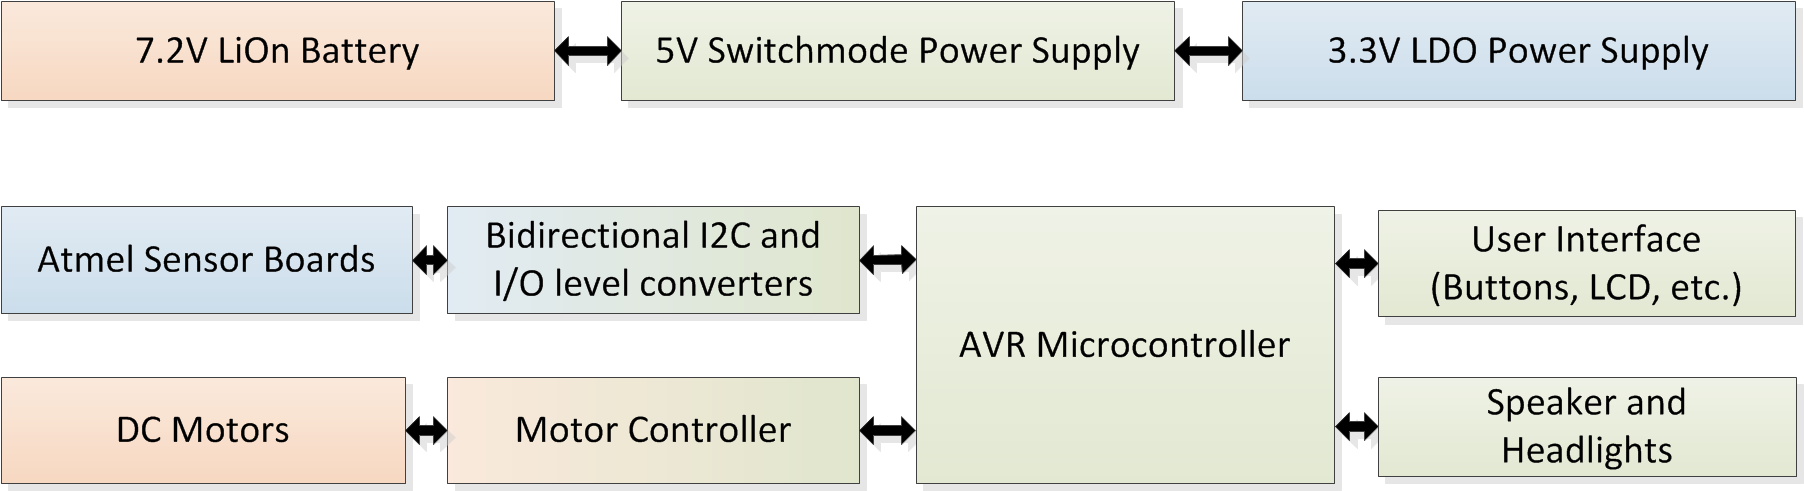
\includegraphics[width=140mm]{HardwareBlockDiagram.png}
	\rule{35em}{0.5pt}
	\caption[Hardware Block Diagram]{Robot Hardware Block Diagram}
	\label{fig:robotblockhw}
\end{figure}

\FloatBarrier
\subsection{Microprocessor}

Due to the author's familiarity with the Atmel line of \textit{AVR} branded microcontrollers, one of the available models in this line-up was chosen to serve in the robot as the main processor, the AT90USB1287. This 8-bit microcontroller contains 128KB of non-volatile FLASH memory for program storage, 4KB of non-volatile EEPROM for user application parameter storage and 8KB of internal SRAM for scratch memory. A 16MHz clock (provided by an external crystal) was selected for the design as this offered the fastest possible speed the chip was capable of, while still allowing the hardware USB host controller inside the chip to function normally. As a trade-off, this higher clock speed put a constraint on the main logic level voltage; at 16MHz, the AVR microcontroller required 5V to be within the datasheet's specifications \cite{at90usb1287}.

As the AT90USB1287 and associated USB components are difficult to source in single quantities at reasonable prices, the use of a commercial breakout module containing this chip was selected instead: the \textit{Micropendous-A} board (see Figure \ref{fig:micropendous}). This board contains the surface mount AVR microcontroller and associated USB components, along with an external 128KB SRAM chip attached to the AVR's external memory bus interface \cite{micropendous}. As the Bluetooth stack required a large temporary buffer for incoming fragments, the selection of this board proved ideal for the intended purpose.

\begin{figure}[tbph]
	\vspace{1em}
	\centering
		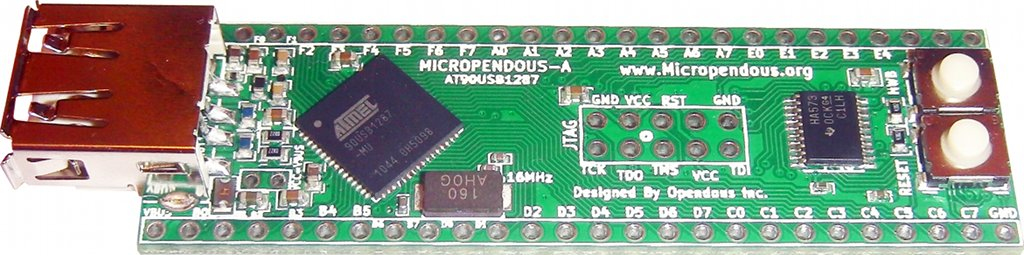
\includegraphics[width=100mm]{MicropendousA.jpg}
	\rule{35em}{0.5pt}
	\caption[Micropendous-A Board]{The Micropendous-A Board (Image courtesy \textit{Opendous Inc.})}
	\label{fig:micropendous}
\end{figure}

\FloatBarrier
\subsection{Primary Power Supply}

As the vast majority of the robot's hardware operated at a fixed 5V level, a power supply was required to reduce the Lithium Ion battery's raw 7.2V (nominal) voltage down to the 5V level needed to power the various components. Due to the use of battery power in the project, reducing power consumption where possible was a large concern; thus, a switch-mode design was chosen for maximum voltage conversion efficiency. A conventional linear regulator was considered for the design, but rejected due to the prohibitively large amount of power this would waste (approximately .45W, assuming an average 200mA operating current).

The regulator selected for the project was the LM2595-5.0, a fixed-function switch-mode regulator capable of outputting a fixed 5V rail at loads of up to 3A \cite{lm2595}. While the robot design would not consume even a fifth of this power, the overhead in the specifications ensured that the power supply would remain robust and the output within the tolerances of the system components regardless of the load demanded. The exact schematic used in the final robot power supply design (see Figure \ref{fig:mainpowersupply}) was taken from the regulator component's datasheet to ensure correct operation.

\begin{figure}[tbph]
	\centering
		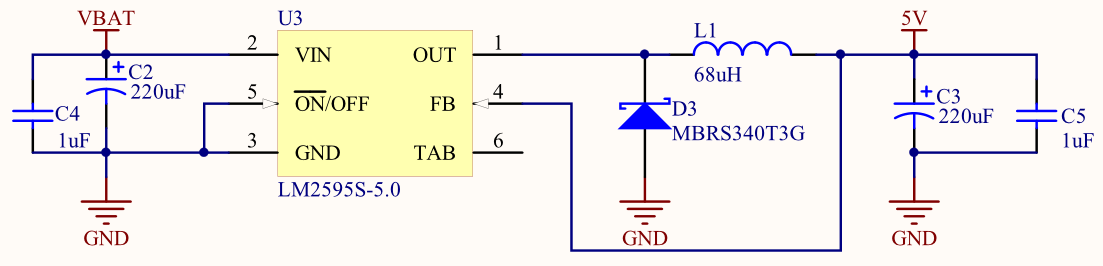
\includegraphics[width=140mm]{MainPowerSupply.png}
	\rule{35em}{0.5pt}
	\caption[Main Power Supply Schematic]{Schematic of the robot's main 5V switch-mode power supply.}
	\label{fig:mainpowersupply}
\end{figure}

\FloatBarrier
\subsection{User Interface}

For interaction with the user, the robot contains several components, detailed below.

\FloatBarrier
\subsubsection{RGB Status LED}

For primary status indication, a surface mount RGB LED indicates the current status of the robot. Due to a lack of free PWM channels on the AVR microcontroller, the three LED sub-components are wired directly to standard GPIO ports. While this design prevented PWM fading of the individual LED subcomponents to produce a many-bit custom colour from the LED, a three bit colour space is possible giving a total of 8 possible colour states (see Table \ref{tab:rgbcolours}). For the purposes of the created robot, this is in practice more than enough for basic status indication.

\begin{table}[H]
	\begin{center}
		\begin{tabular}{ | l | l | l | l |}
			\hline
			\textbf{R}	& \textbf{G} & \textbf{B} & \textbf{Output Colour} \\ \hline

			0 & 0 & 0 & Off		\\ \hline
			0 & 0 & 1 & Blue	\\ \hline
			0 & 1 & 1 & Cyan	\\ \hline
			0 & 1 & 0 & Green	\\ \hline
			1 & 1 & 0 & Magenta	\\ \hline
			1 & 0 & 0 & Red		\\ \hline
			1 & 0 & 1 & Yellow	\\ \hline
			1 & 1 & 1 & White	\\ \hline
		\end{tabular}
		\caption[RGB LED Colour Table]{List of the possible output colours of the RGB LED, from the possible binary channel inputs.}
		\label{tab:rgbcolours}
	\end{center}
\end{table}

To achieve a somewhat uniform brightness, the three LEDs were adjusted with current limiting resistors to consume an equal amount of current (approx. 5mA) despite differing forward voltages. As the RGB status LED shares the same I/O pins as the microcontroller's JTAG port for programming and debugging, the RGB LED's common anode was connected via a removable wire link (see Figure \ref{fig:rgbwirelink}) to ensure that it could be taken out-of-circuit if it proved to interfere with the external hardware debugger during development.

\begin{figure}[tbph]
	\centering
		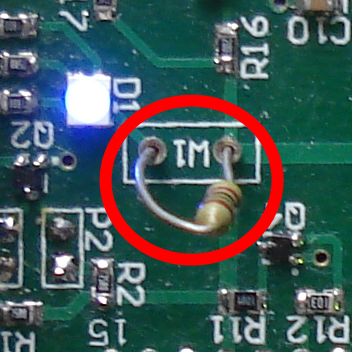
\includegraphics[width=40mm]{RGBWireLink.png}
	\rule{35em}{0.5pt}
	\caption[Close-up of the RGB LED's Removable Wire Link]{Close-up of the removable wire link used to disable the RGB status LED to prevent conflicts with the JTAG lines during programming/debugging.}
	\label{fig:rgbwirelink}
\end{figure}

\FloatBarrier
\subsubsection{LCD Display}

For situations where more information needs to be communicated to the user than is possible via the RGB status LED, a 16x2 Alphanumeric LCD display---compatible with the well known Hitachi HD44780 chipset---was added to the design. Due to the limited number of GPIO pins available on the microcontroller, the LCD was wired in 4-bit mode, with the lower 4 data pins on the LCD being wired directly to ground (see Figure \ref{fig:lcdschematic}). While this doubled the time required to send a byte to the LCD (as bytes then need to be split into a pair of 4-bit nibbles) the high speed of the processor meant that in practice this had little or no effect to the overall speed of the system.

The LCD backlight was wired through a driver transistor to a spare PWM channel on the AVR microcontroller, allowing for 8-bit PWM brightness control to reduce power consumption of the backlight when not in use. As the LCD display's LED backlight had a nominal forward voltage of around 3V, a 10\ensuremath{\Omega} resistor was used to limit the maximum drive current to around 200mA.

\begin{figure}[tbph]
	\centering
		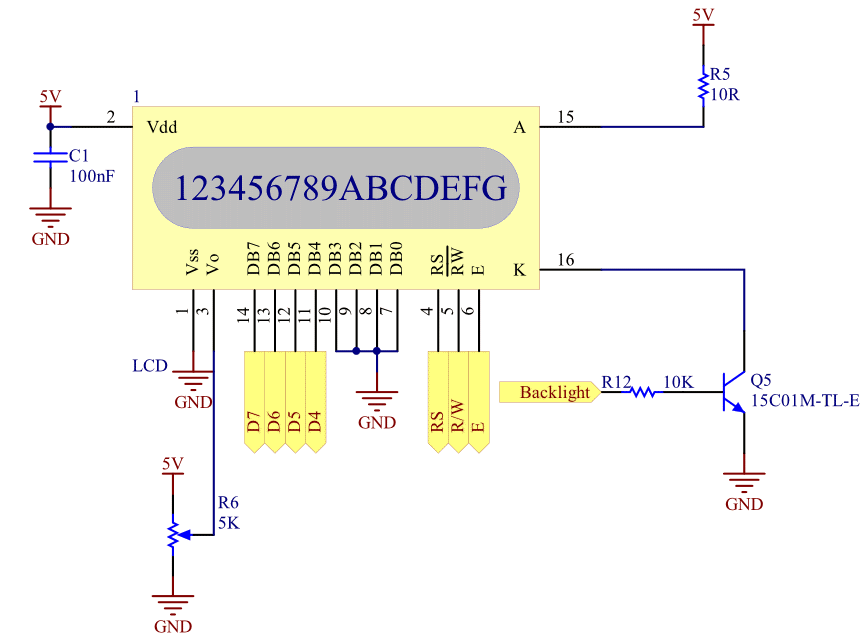
\includegraphics[width=100mm]{LCDSchematic.png}
	\rule{35em}{0.5pt}
	\caption[LCD Display Schematic]{Schematic of the LCD connections, showing the 4-bit LCD data bus mode and backlight driver transistor.}
	\label{fig:lcdschematic}
\end{figure}

\FloatBarrier
\subsubsection{Buttons}

A pair of standard PCB round buttons were added to the design, for user input. These buttons were wired directly to the microcontroller's GPIO pins; internal pull-up resistors in the microcontroller takes care of maintaining a defined logic level on the pins when the buttons are released, while software handles the debouncing of the button signals.

\FloatBarrier
\subsection{Headlights}

To provide illumination of the area immediately ahead of the robot, a pair of high intensity wide viewing angle white LEDs were added to the schematic, connected to a single common driver transistor and driven by a GPIO pin of the microcontroller. To ensure maximum illumination, the LEDs were driven at just under their full 20mA rating when turned on. These ``headlights'' were then mounted on the front of the robot chassis.

\FloatBarrier
\subsection{Speaker}

A small PCB Piezo speaker was added to the robot, in order to provide both audio feedback for important events (such as Bluetooth connections and disconnections) as well as to act as a miniature horn to attract the attention of any organic obstacles to encourage them to move away from the robot's line of motion. Rather than mounting the speaker directly onto the PCB, it was determined that a better location was in between the two frontal headlight LEDs, with the speaker then connected back to the PCB via flyleads. This arrangement made the directional speaker point in the orientation most suited to a car horn, i.e. towards the front of the robot (see Figure \ref{fig:robotspeaker}).

\begin{figure}[tbph]
	\centering
		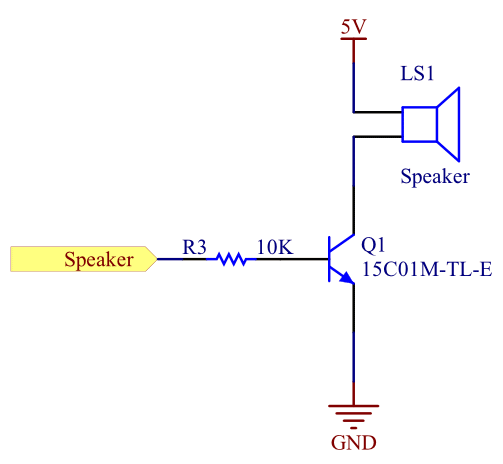
\includegraphics[width=55mm]{SpeakerSchematic.png}
		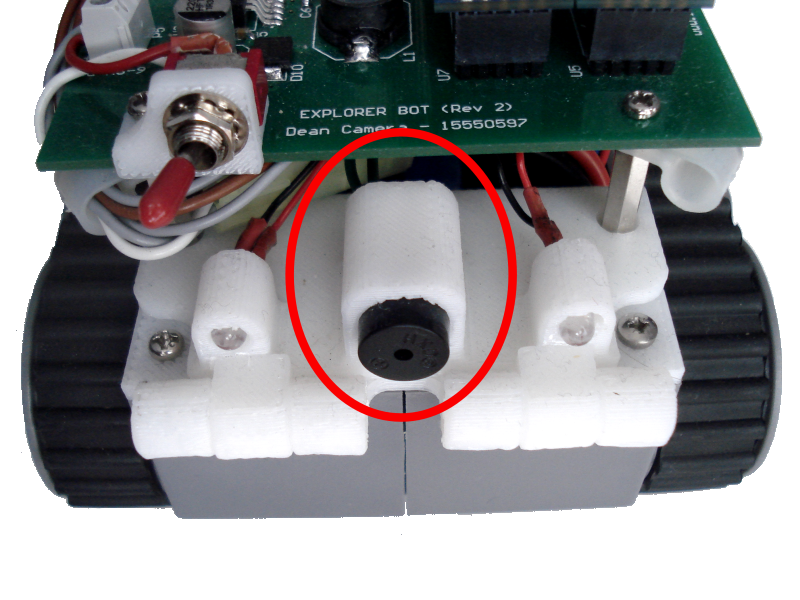
\includegraphics[width=60mm]{RobotFront.png}
	\rule{35em}{0.5pt}
	\caption[Speaker Schematic and Mounting Photo]{Schematic of the robot's piezo speaker (\textit{left}) and photo showing the mounting in the robot prototype (\textit{right}).}
	\label{fig:robotspeaker}
\end{figure}

To drive the speaker, a standard NPN transistor was employed to provide sufficient current, driven from an 8-bit PWM timer output GPIO pin of the AVR microcontroller.

\FloatBarrier
\subsection{Motor Controller}

While the plastic hobbyist ``tank'' style robot base selected for the prototype robot contained a pair of 6V DC motors stock from the factory, it did not contain a motor control system; implementation of a suitable motor control circuit was thus required as part of the project. To prevent motor noise from being injected back into the main 5V power supply used by the sensitive microcontroller, the motors were instead powered directly from the raw battery voltage. By directly powering the motors from the system battery, the main 5V logic power bus could remain relatively undisturbed by the potentially large current spikes caused by the switching on and off of the motors under load. This design had the additional benefit of a reduced total power draw on the main power supply, reducing wasted power due to the supply's non-perfect efficiency and prolonging the operating time of the robot on a fresh battery.

As the raw battery voltage (7.2V nominal) was higher than the motor's 6V maximum, a PWM circuit was thus designed so that the average power delivered to each motor would prevent the motor from burning out during use. While not used in the final robot firmware, the use of variable duty cycle PWM drive signals to the motor would allow for additional speed control of the robot's motors without a corresponding loss of torque.

The motor controller design used in the project centered around the well-known conventional L298N Dual Channel Full H-Bridge Driver IC, notable for its high current drive capabilities and low-voltage logic level drive input support (see Figure \ref{fig:hbridge}) \cite{l298}. Originally the L298D variant was selected due to its convenient internal flyback diodes, however at the time of parts ordering a cheap source for the part could not be found. Unfortunately, the original PCB design did not allow for the possibility of adding external flyback diodes, resulting in the need for a second revised PCB manufacturing run to add in space for the missing components (see Figure \ref{fig:flybackdiodes}). Due to space constraints, the L298N's current sensing capabilities for motor stall detection were not used.

To correctly drive the L298N's PWM inputs, it was necessary to construct a logically inverted version of the PWM signal from the main microprocessor, which would be fed into the L298's channel compliment pin in order to correctly switch on and off the correct portions of the internal H-Bridge circuit. As the chosen microcontroller did not contain enough free pins for this function, a pair of external inverters were constructed out of discrete parts (see Figure \ref{fig:transistorinverter}). This basic logic inverter was used to invert each of the two motor PWM signals for the H-Bridge IC.

\begin{figure}[tbph]
	\centering
		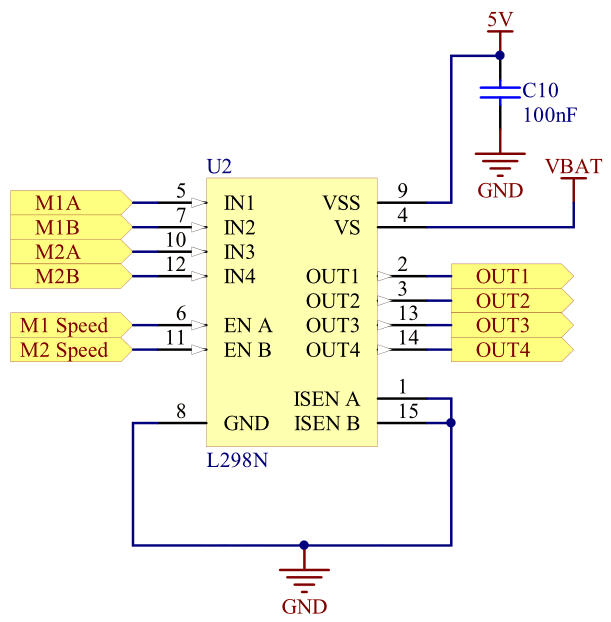
\includegraphics[width=55mm]{HBridgeSchematic.png}
	\rule{35em}{0.5pt}
	\caption[Motor H-Bridge Schematic]{Schematic of the L298N H-Bridge circuit used.}
	\label{fig:hbridge}
\end{figure}

\begin{figure}[tbph]
	\centering
		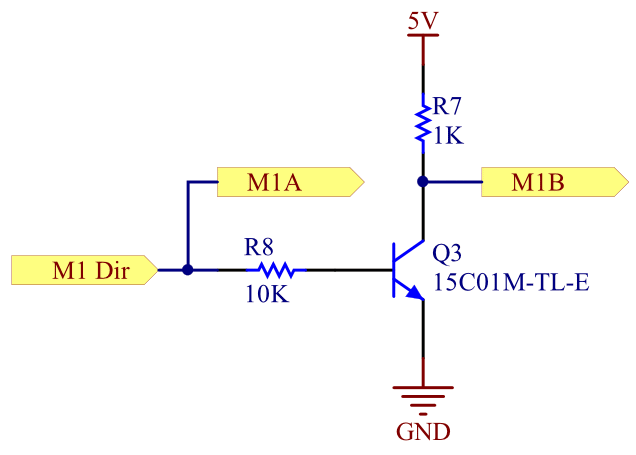
\includegraphics[width=55mm]{TransistorInverter.png}
	\rule{35em}{0.5pt}
	\caption[Transistor Inverter Schematic]{Schematic of one of the transistor inverters used to generate the compliment of the PWM signal used by the motor H-Bridge.}
	\label{fig:transistorinverter}
\end{figure}

\begin{figure}[tbph]
	\centering
		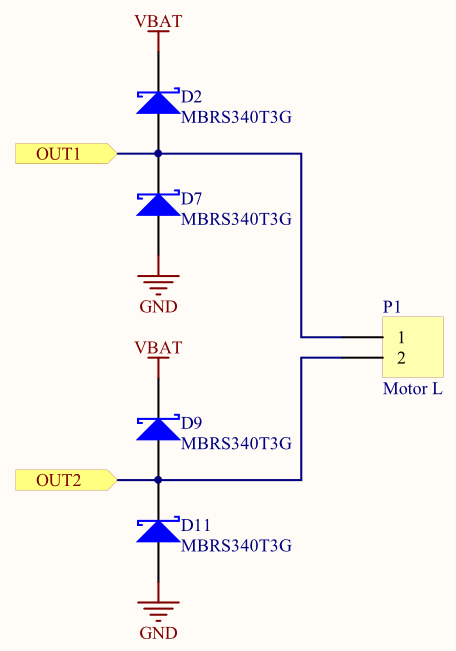
\includegraphics[width=55mm]{FlybackDiodeSchematic.png}
		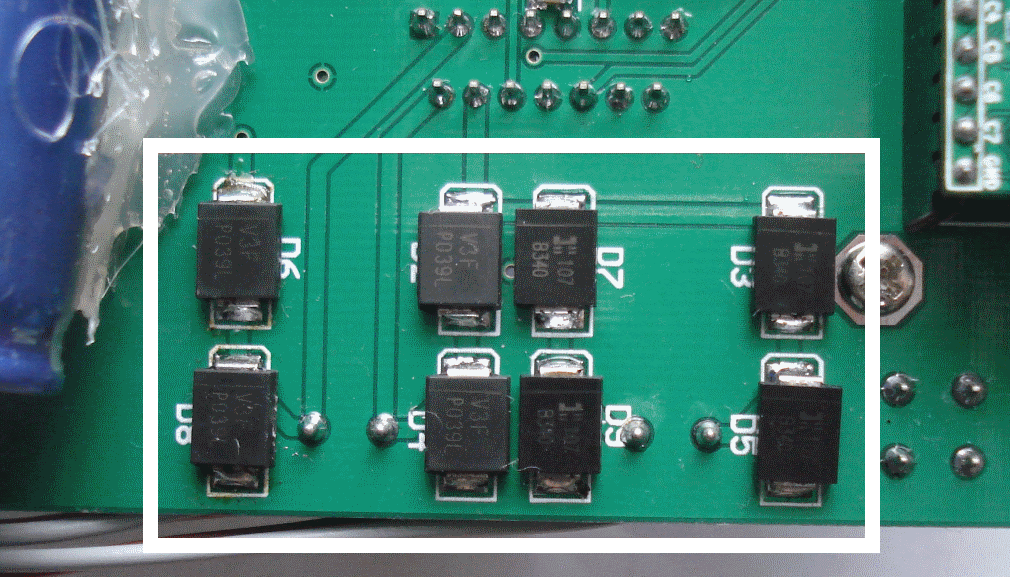
\includegraphics[width=80mm]{FlybackDiodes.png}
	\rule{35em}{0.5pt}
	\caption[Motor Flyback Diodes]{Partial schematic \textit{(left)} and photo \textit{(right)} of the external flyback diodes added in the second PCB revision to the robot's motors.}
	\label{fig:flybackdiodes}
\end{figure}

\FloatBarrier
\subsection{Sensors}

To provide a measure of feedback from the robot, a number of sensors were added to the design. These sensors, when attached, would allow for the robot's environment to be logged and (potentially) reacted to.

\FloatBarrier
\subsubsection{Sensor Power Supply}

While the main system logic and user interface components run from the main switch-mode 5V power supply, the sensor boards were required to run at a fixed 3.3V level, without the possibility of conversion to suit the higher rail voltage.

For this reason, and to reduce the amount of noise on the sensor power supply for maximum precision, a decision was made to add a secondary power supply, running from the 5V rail, to step down the voltage to the 3.3V required by the sensor boards. For best results, an ADP3308 Low Dropout (LDO) style regular was used as this provided both low output rail noise and minimal wasted power \cite{adp3308}.

\FloatBarrier
\subsubsection{Level Converters}

Due to the differing bus voltages between the sensor boards (3.3V) and the main processor (5V), level conversion of the I\textsuperscript{2}C bus and sensor interrupt/control lines was required. While only a unidirectional buffer was strictly needed for each of the sensor interrupt/control lines, it was decided to use a bidirectional converter to ease the board routing.

Initially, only an ADG3308 8-channel Bidirectional Level Converter IC was used, for both the sensor interrupt/control lines, as well as the I\textsuperscript{2}C bus. However, after further analysis it was discovered that the level translator would not meet the timing requirements of the I\textsuperscript{2}C bus \cite{adg3308}, necessitating the addition of a secondary dedicated Texas Instruments PCA9306 fixed function I\textsuperscript{2}C bus level converter IC in the second revision of the board. As a bonus, the use of the later chip allowed the I\textsuperscript{2}C bus to be driven at the ``Fast'' I\textsuperscript{2}C speed of 200KHz for minimal latency and maximum throughput.

Unusually, the ADG3308 level converter IC required that its enable pin (located on the low voltage side of the translator) be connected to the higher logic level for the chip to become active (see Figure \ref{fig:ADG3308schematic}). This odd placement of the enable pin resulted in a non-optimal breaking of the ground plane underneath the chip to accommodate the required route, as the space between the chip package pins on the top layer was used to carry the 3.3V power bus to the sensor boards (see Figure \ref{fig:ADG3308routing}).

\begin{figure}[tbph]
	\centering
		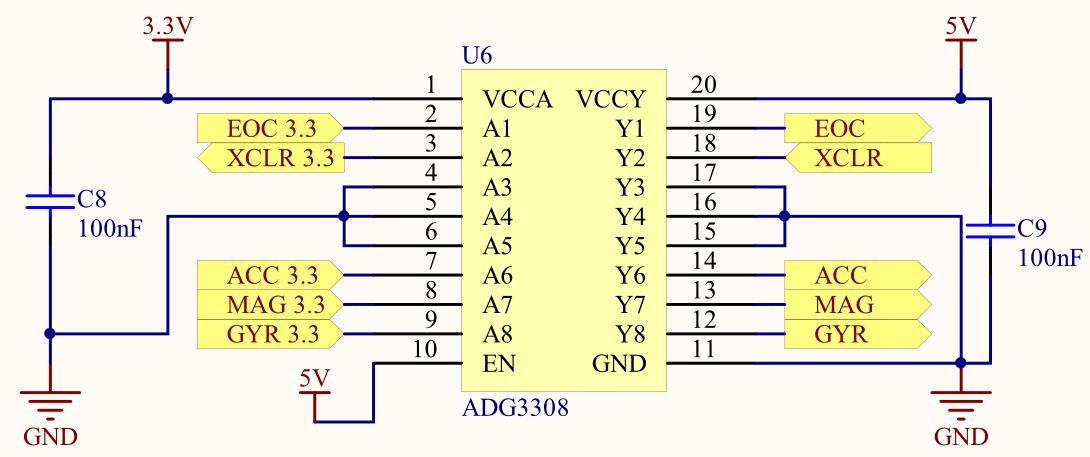
\includegraphics[width=120mm]{LevelTranslatorSchematic.png}
	\rule{35em}{0.5pt}
	\caption[Bidirectional Level Translator Schematic]{Schematic of the ADG3308, showing the unusual placement of the VCC-Y level active high enable pin.}
	\label{fig:ADG3308schematic}
\end{figure}

\begin{figure}[tbph]
	\centering
		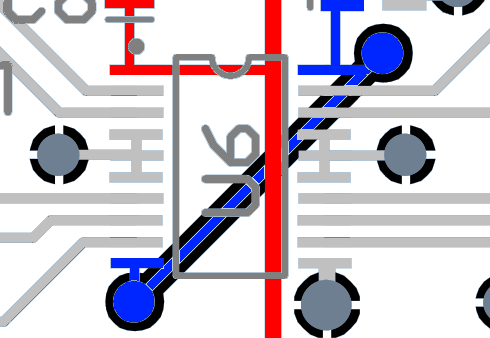
\includegraphics[width=50mm]{LevelConverterRouting.png}
	\rule{35em}{0.5pt}
	\caption[Bidirectional Level Translator Routing]{Routing of the ADG3308, showing the 3.3V bus (red) and 5V enable (blue) routes.}
	\label{fig:ADG3308routing}
\end{figure}

The board routing complexity was reduced slightly by swapping the functions of the PCA9306 bus level translator's SDA and SCL pins (see Figure \ref{fig:PCA9306schematic}) on both sides of the IC; this modification (allowable as indicated in the device's datasheet \cite{pca9306}) prevented the need to introduce additional board vias and longer trace routes.

\begin{figure}[tbph]
	\centering
		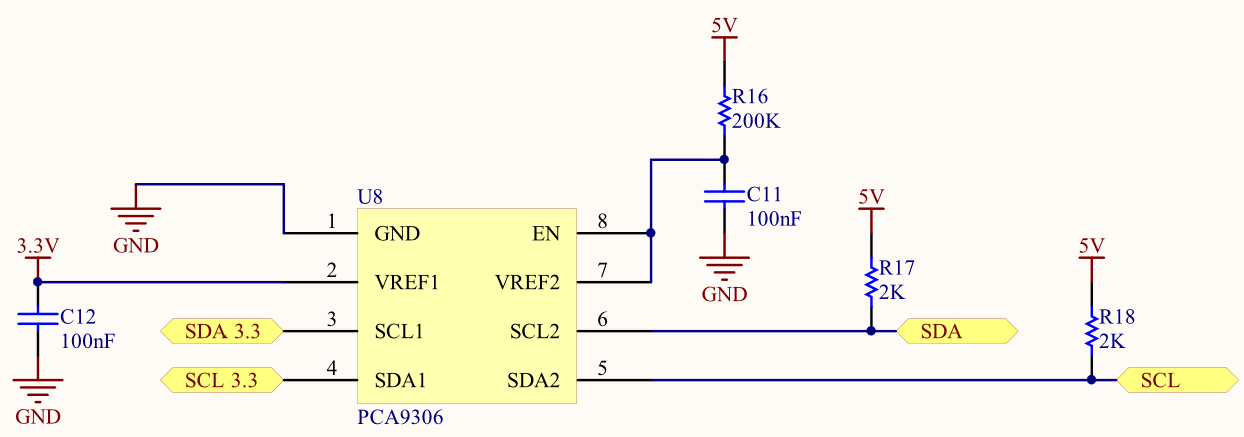
\includegraphics[width=140mm]{I2CTranslatorSchematic.png}
	\rule{35em}{0.5pt}
	\caption[I\textsuperscript{2}C Level Translator Schematic]{Schematic of the PCA9306, showing the swapped SDA and SCL pin functions.}
	\label{fig:PCA9306schematic}
\end{figure}

\FloatBarrier
\subsubsection{Atmel Sensor Boards}

By designing the robot around a pair of commercially available Atmel sensor boards for environmental feedback, the design of the robot was considerably simplified and the total unit cost lowered. The \textit{Atmel Pressure One} board contains a Bosch BMP085 Pressure Sensor IC for air pressure sensing \cite{pressureone}, while the Atmel \textit{Inertial One} contains a 3-Axis ITG3200 Gyroscope, 3-Axis BMA150 Accelerometer and 3-Axis AK8975 Compass IC (see Figure \ref{fig:atmelsensorboards}) \cite{inertialone}. As several of the sensors also contain a digital temperature sensor in addition to the primary sensor (for calibration and stability feedback) this functionality was also used by the robot to measure the environmental temperature in real time.

Each sensor IC is driven by the main microcontroller of the robot over the level converted I\textsuperscript{2}C bus and one or more digital interrupt/control lines. The Atmel sensor board modules all use an identical form factor, with one standard .1" 2x5 female header located at one end of the board reserved for the mounted sensor's digital I/O pins, and another located at the opposite end of the board reserved for analogue sensor pinouts. As none of the sensor boards used contained analogue sensor outputs, the second female header consisted only of non-connected pins, and a matching male header was placed on the board for mechanical stability only.

\begin{figure}[tbph]
	\centering
		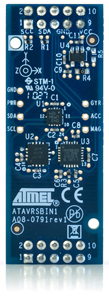
\includegraphics[height=70mm]{Inertial1.jpg}
		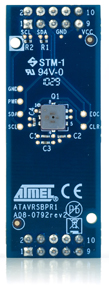
\includegraphics[height=70mm]{Pressure1.jpg}
	\rule{35em}{0.5pt}
	\caption[Atmel Sensor Boards]{The Atmel \emph{Inertial One} (left) and \emph{Pressure One} (right) Sensor Boards \cite{pressureone} \cite{inertialone}}
	\label{fig:atmelsensorboards}
\end{figure}

\section{Final PCB Design}

The final revision of the robot PCB is shown in Figure \ref{fig:rev2pcb}. The layout of the various hardware sections on the PCB was kept as modular as possible, and confined to the top layer where practical to ensure a good ground plane on the bottom PCB layer.

\begin{figure}[tbph]
	\centering
		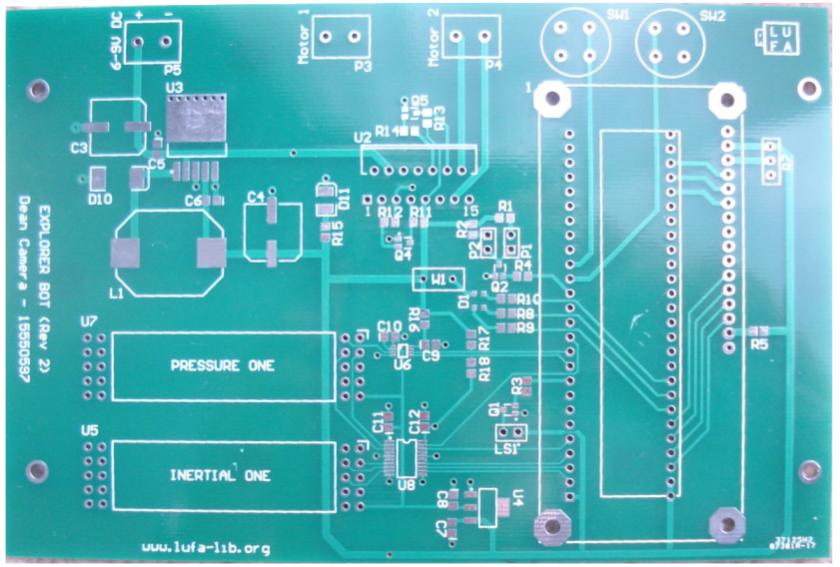
\includegraphics[width=95mm,angle=90]{PCBRev2Front.jpg}
		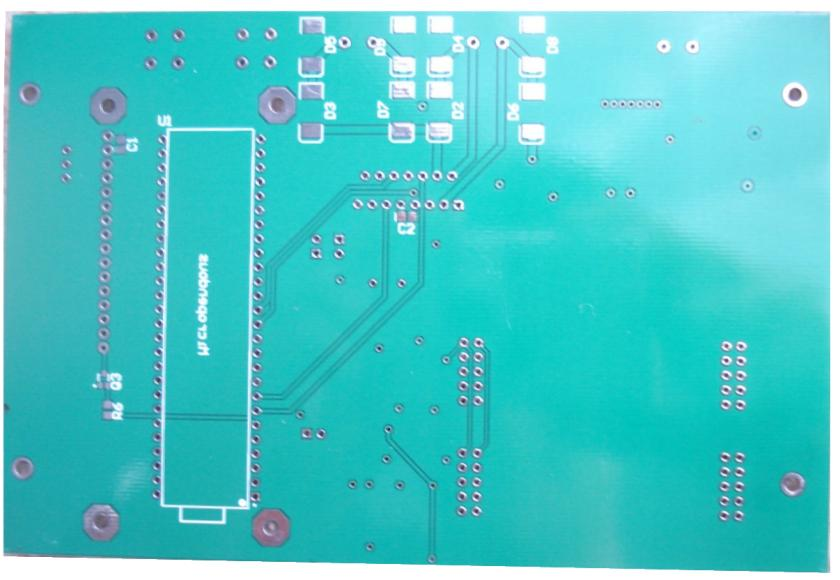
\includegraphics[width=95mm,angle=90]{PCBRev2Back.jpg}
	\rule{35em}{0.5pt}
	\caption[Final Revision PCB]{Photos of the final revision PCB top side (\textit{left}) and bottom side (\textit{right}) used in the robot prototype.}
	\label{fig:rev2pcb}
\end{figure}

The PCB artwork is shown in Figure \ref{fig:rev2pcbartwork}. Note that the ground layer fill has been removed from the bottom layer for clarity.

\begin{figure}[tbph]
	\centering
		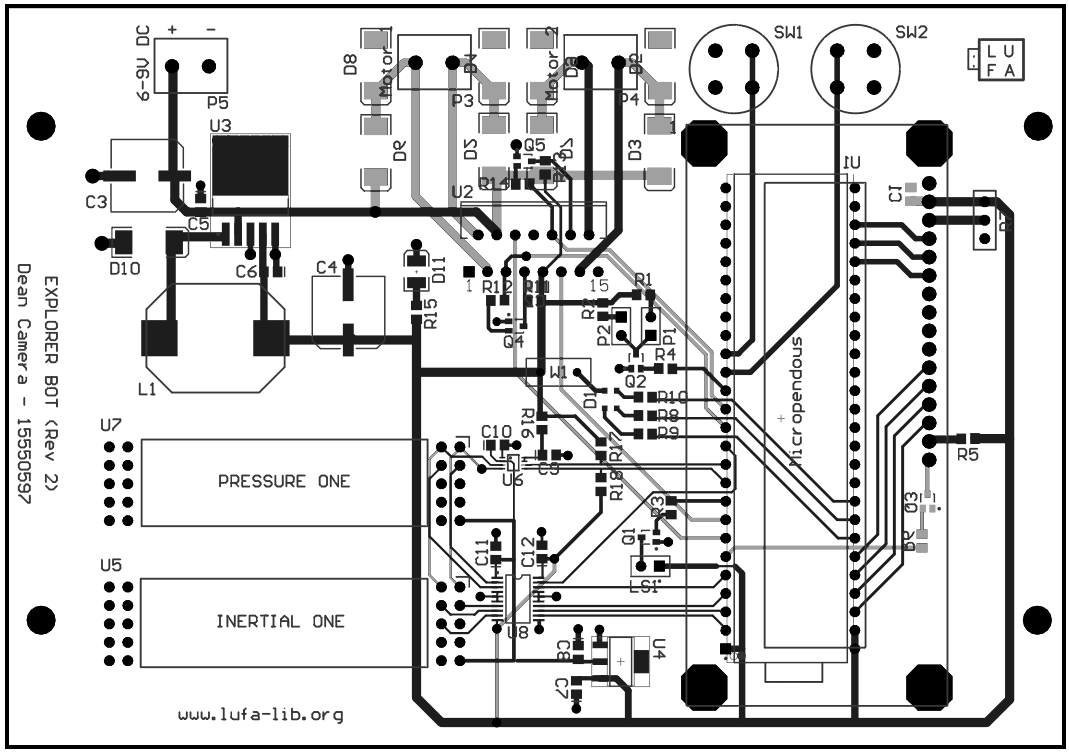
\includegraphics[width=180mm,angle=90]{PCBArtwork.png}
	\rule{35em}{0.5pt}
	\caption[PCB Artwork]{Artwork of the final revision PCB, showing both the top (\textit{black}) and bottom (\textit{gray}) layers.}
	\label{fig:rev2pcbartwork}
\end{figure}
